\section{Introduction}
\label{sec:introduction}

Large language model (LLM) agents are increasingly expected to carry out workflows that combine information gathering, tool use, and multistep reasoning. Such work often contains complementary subtasks whose outputs must be integrated into a complete solution. Multi-agent systems distribute these subtasks across agents, supporting specialized execution and collaboration through conversations or role-based workflows, as exemplified by AutoGen~\citep{wu2023autogen} and MetaGPT~\citep{hong2023metagpt}. When independent subtasks run concurrently, multiple agents can also make progress on different parts of the same task, motivating recent efforts to train parallel agent systems such as Parallel-Agent Reinforcement Learning (PARL)~\citep{kimiteam2026kimik25}.

Realizing these benefits requires effective \emph{orchestration}. An orchestrator must identify useful subgoals, delegate them to workers, schedule execution around their dependencies, and integrate the returned results. For example, workers can retrieve evidence from independent sources in parallel, but a comparison must wait for the relevant findings. Decomposing a task too finely increases coordination overhead, whereas unnecessary serialization leaves independent work waiting. Effective orchestration therefore requires choosing an appropriate task decomposition while preserving correctness.

Many multi-agent frameworks implement coordination through prompts and predefined workflows, relying on the underlying model's existing capabilities. Although recent methods train orchestration with reinforcement learning, including PARL~\citep{kimiteam2026kimik25} and ParaManager~\citep{yuan2026paramanager}, scaling this training presents two challenges. \emph{First, training needs executable tasks with useful serial dependencies and parallel branches.} These structures let the policy practice deciding what to delegate and when to combine results. \emph{Second, terminal success alone provides limited feedback on incomplete executions.} A rollout that obtains most of the required evidence but omits one result can receive the same zero reward as one that makes no useful progress. If all rollouts in a GRPO group fail under a binary reward, their centered advantages are zero. Process feedback can distinguish such trajectories by the progress they actually make, providing a learning signal before complete solutions are sampled.

\begin{figure}[t]
  \centering
  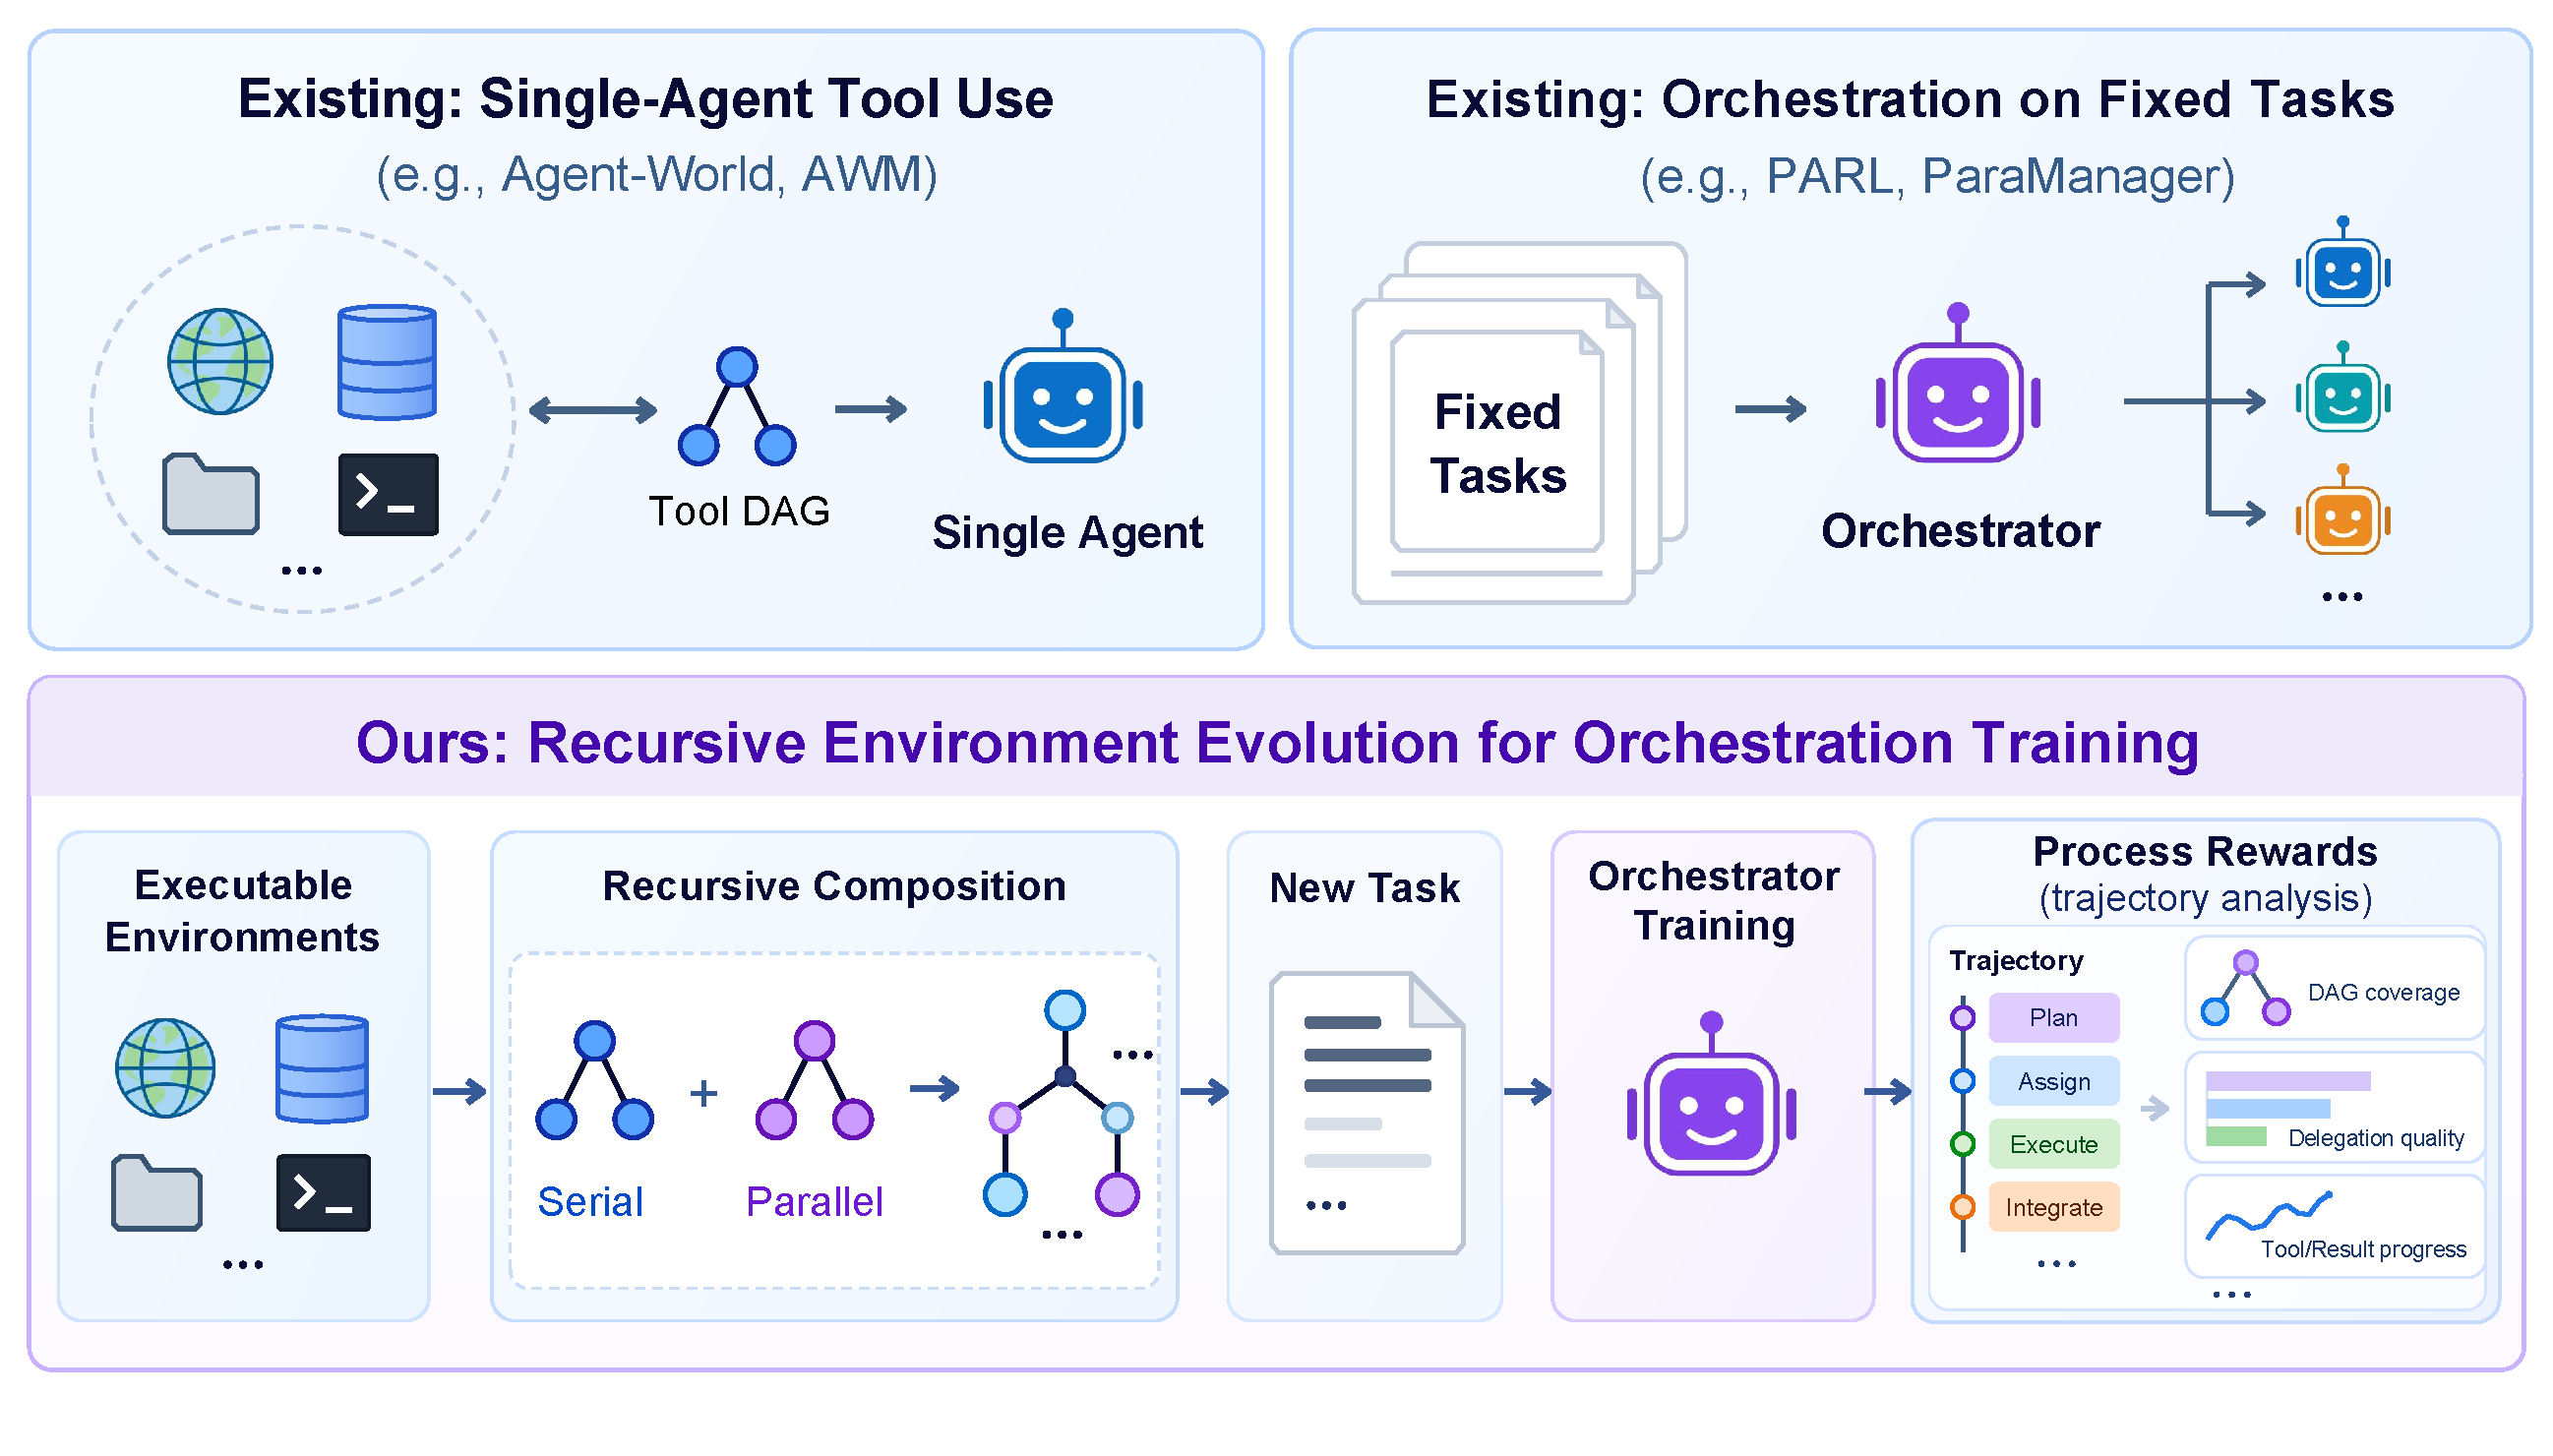
\includegraphics[width=0.75\linewidth]{figures/figure1.pdf}
  \caption{\textbf{Environment requirements for orchestration training.} Executable tools, state, and a verifier support tool-use learning (left). Orchestration tasks expose subgoals linked by serial dependencies or parallel branches (center), supporting delegation and result integration (right). The workflows illustrate training requirements.}
  \label{fig:environment-requirements}
\end{figure}

Training environments determine which decisions an agent can practice and what feedback it receives. Agent World Model~\citep{wang2026agentworldmodelinfinity}, Agent-World~\citep{dong2026agentworld}, and ToolVerse~\citep{zhou2026toolverse} construct executable tools and verifiable tasks for tool-use training. Building on this setting, MAW focuses on composing functional goals into coherent requests that require coordinating serial dependencies and parallel branches (Figure~\ref{fig:environment-requirements}). The construction must preserve executable interactions and evidence for checking both progress and completion.

We introduce \textbf{Multi-Agent World (MAW)}, a framework that combines recursive environment evolution with reinforcement learning for orchestration (Figure~\ref{fig:maw-overview}). MAW represents reference tool calls and their dependencies as directed acyclic graphs (DAGs), then composes task candidates through serial and parallel operations. Semantic reconstruction turns the candidate graphs into coherent user requests. Executing the reconstructed reference and applying quality gates check feasibility and agreement among the request, answer, and database state. The accepted tasks support training in which an orchestrator assigns roles and subtasks to frozen workers. We combine final outcome verification with process feedback on tool progress, answer coverage, and task organization, and optimize the orchestrator with Group Relative Policy Optimization (GRPO)~\citep{shao2024deepseekmath}.

\begin{figure}[t]
  \centering
  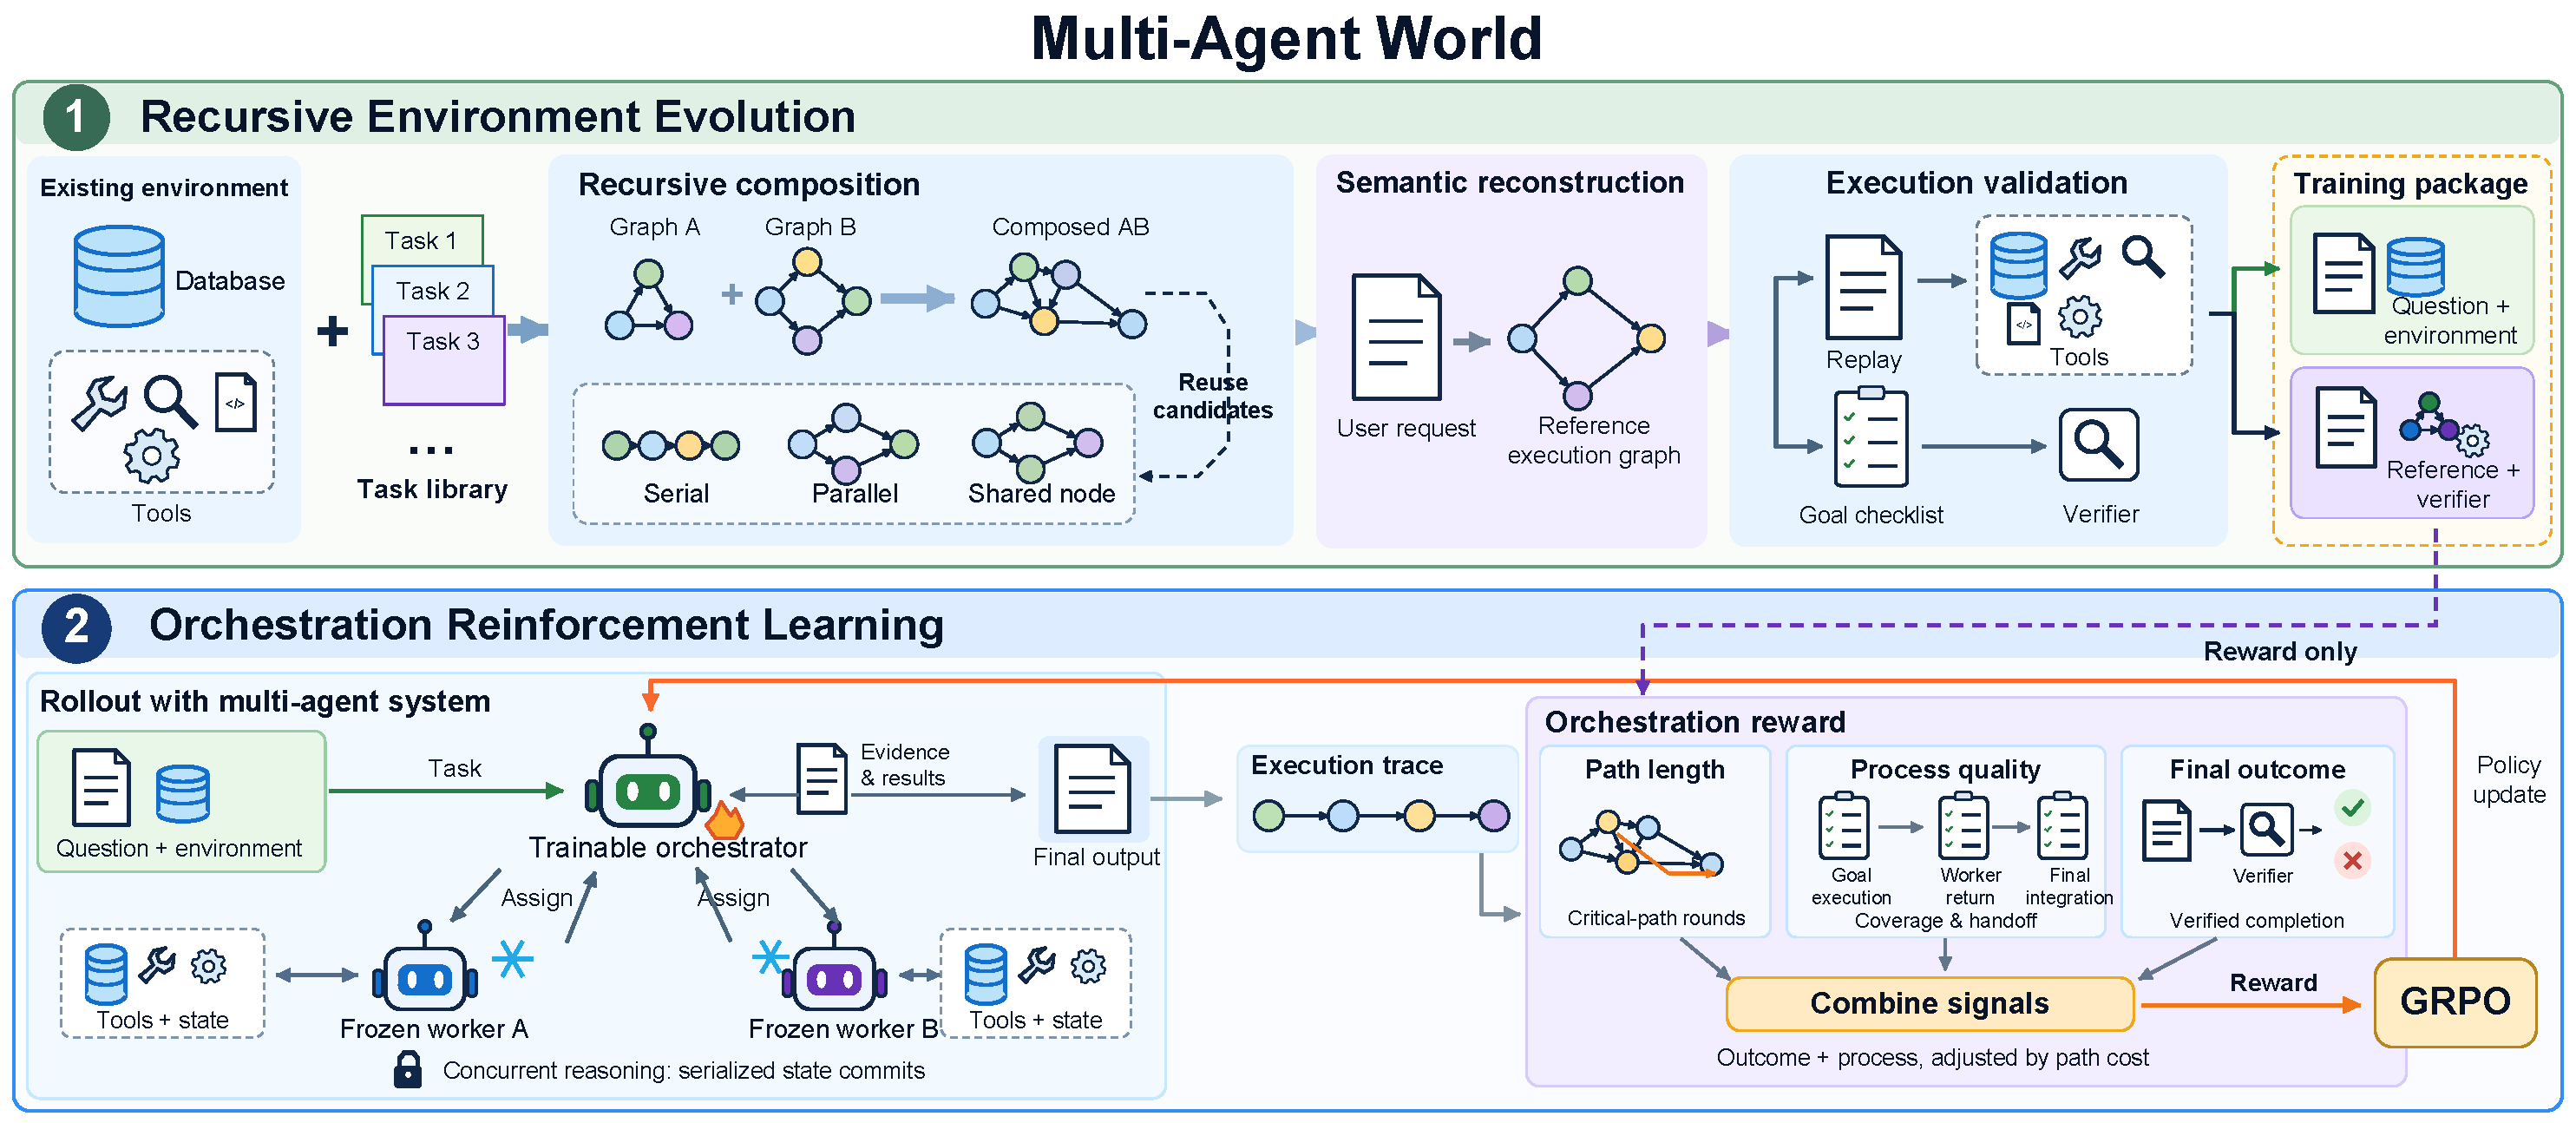
\includegraphics[width=\linewidth]{figures/figure2.pdf}
  \caption{\textbf{Overview of Multi-Agent World.} Task construction connects DAG composition, semantic reconstruction, execution, and quality gates. Accepted tasks provide resettable environments for interaction and hidden references for scoring. The orchestrator dynamically creates and reuses workers, combines their results, and receives a trajectory reward from outcome verification and process feedback. Only the orchestrator is updated.}
  \label{fig:maw-overview}
\end{figure}

Our evaluation examines task construction, transfer to external benchmarks, and the contribution of process feedback. The audited synthesis snapshot contains 2,581 accepted tasks in 539 environments; its comparison with the seed set is reported in Section~\ref{sec:composition}. Controlled training comparisons are designed to separate data-source effects from reward effects. \drafttodo{Report verified benchmark results and ablations; the synthesis counts alone do not establish training gains.}

Our contributions are as follows:
\begin{itemize}
  \item \textbf{Task construction for orchestration training.} We develop serial and parallel DAG composition, semantic reconstruction, and execution-based quality control to construct verifiable tasks within existing environments.
  \item \textbf{Orchestration RL with execution-grounded process feedback.} We combine final answer and database-state verification with feedback on tool progress, answer coverage, and delegated work to train the orchestrator.
  \item \textbf{Evaluation of task construction and orchestration learning.} We compare the seed and synthesized task sets and specify controlled data and reward comparisons. \drafttodo{Replace the planned learning comparisons with their measured findings.}
\end{itemize}
